Nesta seção, será elaborado o Gêmeo Digital do Aeropêndulo. O Gêmeo Digital representa um sistema gráfico computacional que reproduz em tempo real a dinâmica do protótipo. Isso permite a virtualização do Aeropêndulo, possibilitando a observação da mesma dinâmica do sistema físico, agora em um ambiente gráfico computacional 3D. Essa virtualização é viabilizada pela obtenção do estado atual do braço do Aeropêndulo por meio de comunicação serial.

Para o desenvolvimento do Gêmeo Digital, utilizou-se a biblioteca VPython, essa biblioteca possui um conjunto de funções que permite criar objetos 3D capazes de realizar movimentos rotacionais de translacionais, além disso, é possível plotar gráficos em tempo real. A Figura \ref{fig3:image_13_1} ilustra a interface do simulador já finalizado, pode-se observar que a interface é composta de duas partes principais, uma que implementa o ambiente 3D com o Aeropêndulo e a outra gera os gráficos do sinal de referência e de saída.

Com a finalidade de atualizar os estados dos gráficos e a posição angular do gêmeo digital em tempo real a aplicação se comunica com a interface gráfica, subseção \ref{interface_graica}, com isso é possível realizar a atualização dos estados do gráfico assim como do gêmeo digital tendo como entrada os sinais dos estados do protótipo.

\begin{figure}[!h]
	\centering
	\caption{Gêmeo Digital - Simulador com VPython.}
	\efbox{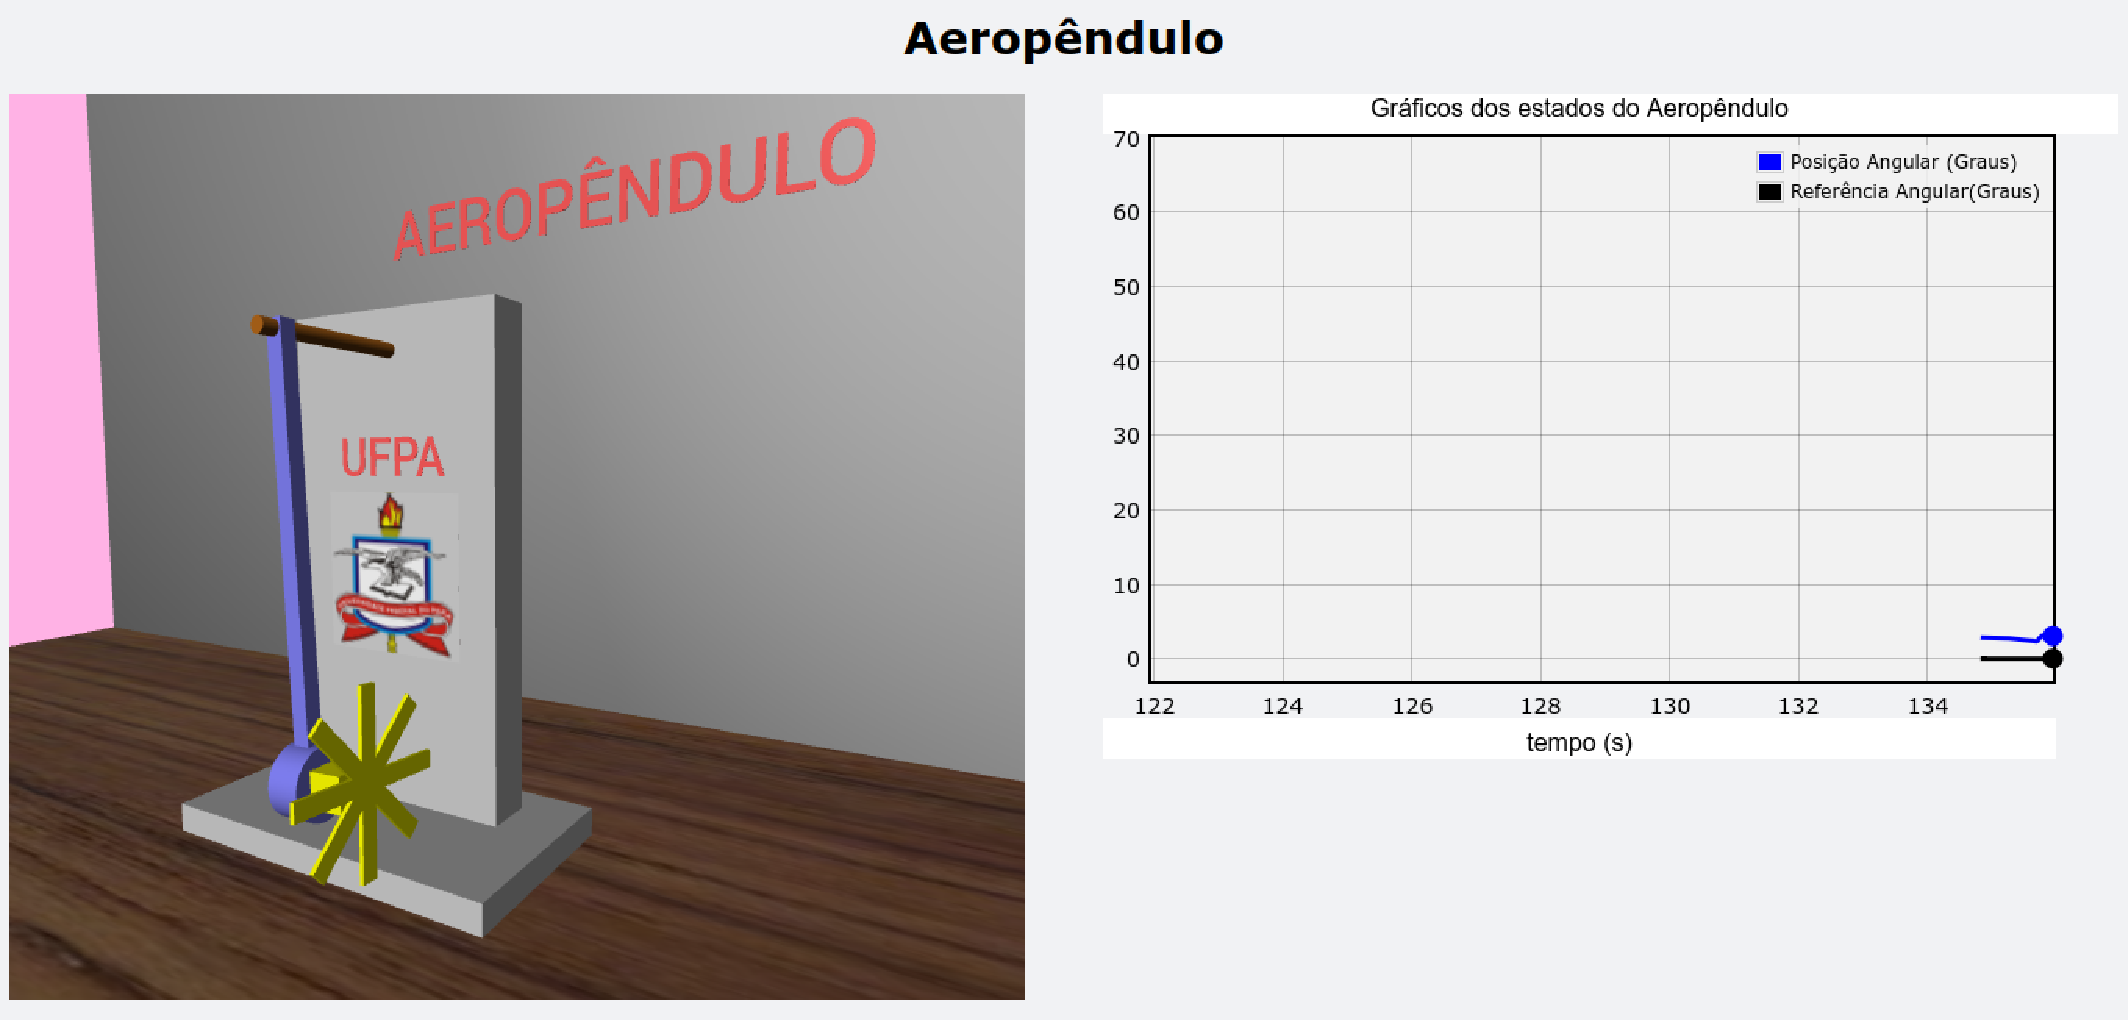
\includegraphics[width=1\textwidth]{Capitulos/3_hardware_softwares/3_figuras/simulador.pdf}}
        \vspace{0.001cm}
	\caption*{Fonte: elaborado pelo autor (2023).}
	\label{fig3:image_13_1}
\end{figure}

% O gêmeo digital do aeropêndulo foi derivado de um projeto que o Autor desse TCC participou, intitulado \textbf{Laboratório Virtual para Sistemas Dinâmicos e Controle na Faculdade de Engenharia Elétrica da UFPA-Tucuruí}, a partir desse projeto foi ...

\newpage
\subsubsection{Biblioteca VPython}

Conforme o site oficial \cite{vpython}, "O VPython, por ser desenvolvido com a linguagem Python, é uma ferramenta versátil para a criação de animações 3D navegáveis. Ele é fácil de aprender e usar, mesmo para pessoas com pouca experiência em programação. No entanto, ele também oferece uma ampla gama de recursos para programadores e pesquisadores experientes."

Ao criar uma simulação com VPython e executá-la, o simulador será renderizado no navegador de internet padrão do sistema operacional.


\subsubsection{Arquitetura do Gêmeo Digital}

Para implementar o simulador a arquitetura do sistema consiste de um módulo para gerar os gráficos de linha e outro para desenhar o simulador 3D, existe um módulo que integra e atualiza os estados dos gráficos de linha e do simulador 3D, a Figura \ref{fig3:image_13} mostra como a estrutura do simulador foi pensada, o último bloco é a interface gráfica, subseção \ref{interface_graica}, responsável por obter os estados do sistema real, com isso, é possível usar a velocidade angular real do protótipo como entrada para o gêmeo digital, isso faz com que a dinâmica do protótipo seja reproduzida no gêmeo digital, além disse, é possível obter os sinais de referência e de saída e atualizar os gráfios que compõem a interface do simulador.

\begin{figure}[!h]
	\centering
	\caption{Diagrama da arquitetura do Gêmeo Digital.}
	\efbox{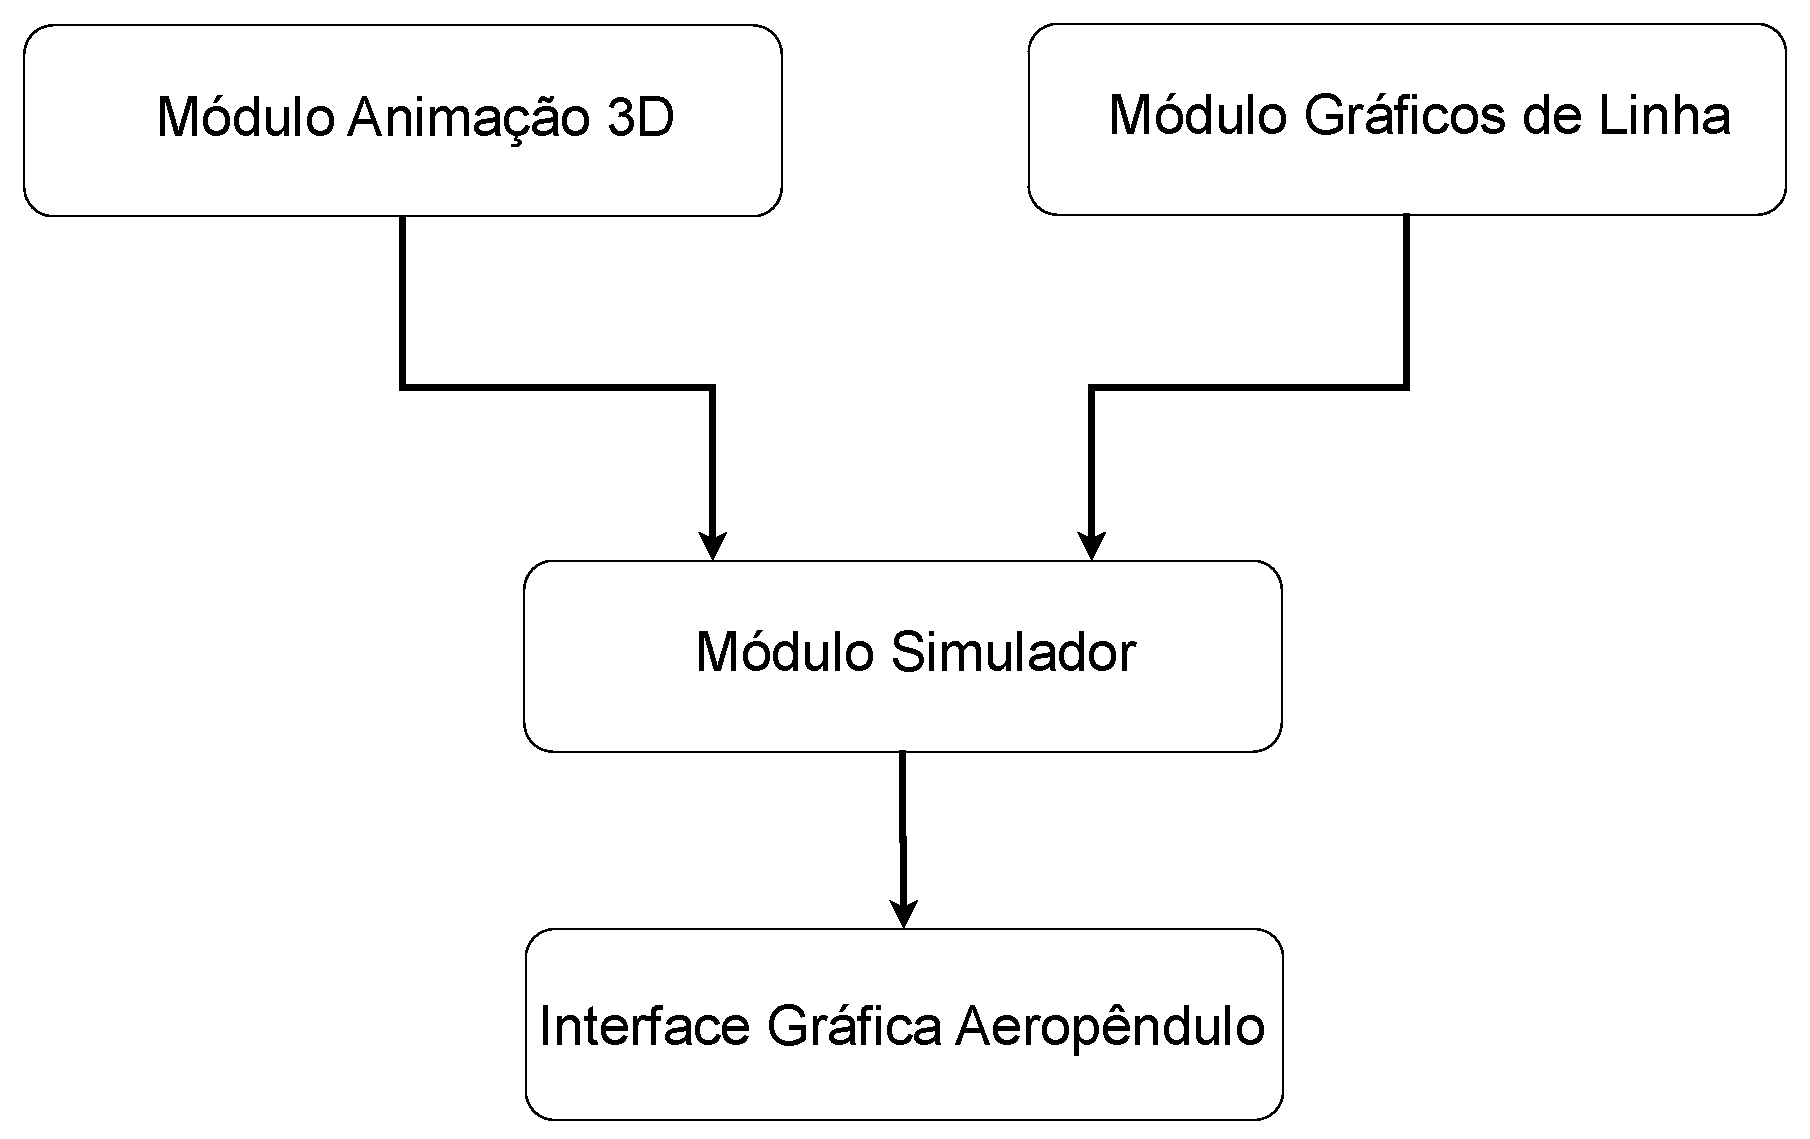
\includegraphics[width=0.55\textwidth, page=1]{Capitulos/3_hardware_softwares/3_figuras/arquitetura_simulador.pdf}}
        \vspace{0.2cm}
	\caption*{Fonte: elaborado pelo autor (2023).}
	\label{fig3:image_13}
\end{figure}


\newpage

O \textbf{Módulo Simulador}, código abaixo, recebe como parâmetro  o \textbf{Módulo Animação 3D} e o \textbf{Módulo Gráficos de Linha}, a partir disso  é implementada uma Classe Python usando a ideia de programação orientada a objetos para realizar a construção tanto da parte gráfica quanto do simulador 2D.

\vspace{0.5cm}

\begin{python}

import vpython as vp

# Modulos do Gemeo Digital desenvolvidos
from .interfaces.graficos_aeropendulo import GraficosInterface
from .interfaces.animacao_aeropendulo import AnimacaoAeropenduloInterface
from .interfaces.simulador import SimuladorInterface


class Simulador(SimuladorInterface):
    def __init__(
            self, graficos: GraficosInterface,
            animacao_aeropendulo: AnimacaoAeropenduloInterface) -> None:
        self.t = 0
        self.t_ant = 0
        self.ts = 0
        self.theta_rad = 0
        self.theta_rad_ant = 0
        self.dtheta_rad = 0
        # Instanciando um objeto AeropenduloAaeropendulo()
        self.animacao_aeropendulo = animacao_aeropendulo

        # Instanciando um objeto para plotagem dos gráficos
        # dinamicos dos estados do Aeropêndulo
        self.g = graficos
        self.graf, self.plot1, self.plot2 = self.g.graficos()  # noqa

    def grau2rad(self, graus):
        return (graus)*(vp.pi/180.0)

    def rotate(self, angle) -> None:
        self.valor_angle = self.grau2rad(angle)
        self.animacao_aeropendulo.aeropendulo.rotate(
            axis=vp.vec(0, 0, 1),
            angle=self.valor_angle,
            origin=vp.vec(0, 5.2, 0))
        self.animacao_aeropendulo.set_posicao_helice(self.valor_angle)

    def atualizar_estados(self, t, theta, ref):
        self.t = t
        self.ts = self.t - self.t_ant
        self.theta_rad = self.grau2rad(theta)
        try:
            self.dtheta_rad = (
                self.theta_rad - self.theta_rad_ant
                )/self.ts
        except Exception as exception:
            print(exception)

        # Atualiza o ângulo do Aeropêndulo
        self.animacao_aeropendulo.aeropendulo.rotate(
                        axis=vp.vec(0, 0, 1),
                        angle=self.dtheta_rad*self.ts,
                        origin=vp.vec(0, 5.2, 0))

        # Animacao da dinamica da Helice
        self.animacao_aeropendulo.update_helice(self.dtheta_rad, self.ts)

        # print(x[1] + interface.valor_angle)
        # Grafico do angulo.
        self.plot1.plot(t, theta)
        # Grafico do sinal de referencia
        self.plot2.plot(t, ref)

        self.t_ant = t
        self.theta_rad_ant = self.theta_rad

\end{python}

Para atualizar a dinâmica do braço do Aeropêndulo do Gêmeo Digital, a classe \textbf{Simulador} é importada no outro software, seção \ref{interface_graica} que implementa a comunicação com o protótipo e obtêm os estados do sistema real, assim é possível atualizar o Gêmeo Digital com dados reais do braço do Aeropêndulo.

Logo, o código desenvolvido para implementar o Gêmeo Digital deve ser importado no código que implementa a Interface Gráfica de Usuário, seção \ref{interface_graica}.